\section{Pregibanje tangent na stožnice}
\label{pogl:stoznice}

\textcolor{red}{A čmo premaknit to poglavje tik pred enačbe?}

Iz didaktičnega vidika zelo zanimivo poglavje nam predstavlja konstrukcije tangent na stožnice s prepogibanjem papirja. Vsebina je tu predstavljena tako, da je bralec najprej povabljen, da vzame list papirja in ga prepogiba po navedenih korakih. Po opažanju, kaj se na papirju pri tem prikaže, preidemo na matematični del, kjer dokažemo, da so prepogibi res tangente na določeno stožnico.

Učitelji matematike so povabljeni, da si pri obravnavi stožnic vzamejo čas in izvedejo spodnje aktivnosti. Dijaki bodo z veliko verjetnostjo presenečeni nad rezultati zgibanja, kar jih lahko bolj motivira za obravnavo geometričnih lastnosti stožnic. Priporočljiva je tudi izvedba ure v računalniški učilnici, kjer lahko vsak dijak z ustreznim programskim orodjem (npr.\ Geogebra) sam poskusi zgraditi opisano konstrukcijo. S tem lahko znanje o stožnicah le še bolj utrdi.

Z origamijem ne moremo konstruirati gladkih krožnih lokov. Kljub temu pa lahko z upoštevanjem določenih korakov konstruiramo premice, ki so tangentne na neko krivuljo. Več takih tangent nam poda nekakšno lomljenko, če pa bi konstrukcije pregibov ponavljali v nedogled, bi v limiti res dobili gladko krivuljo. Pa si poglejmo, kako s prepogibi dobimo obliko stožnic. \textcolor{red}{envelope oz.\ ovojnica:} \url{https://en.wikipedia.org/wiki/Envelope_%28mathematics%29}

\subsection{Krožnica}

% Tega nikjer v literaturi ni in sem sama dodala. Malo preveč osnovno, ma če se obravnava tiste tri stožnice, pa se lahko kar vse, ane.

\textit{\textbf{Aktivnost:} Vzemi list papirja in svinčnik ter na sredi označi točko $S$. Nato drugje označi še točko $A$. Skozi točko $S$ prepogni poljubno premico in na njej označi točko $A'$, da velja $|SA| = |SA'|$. Nato skozi točko $A'$ prepogni pravokotnico na premico $SA'$. To je iskan pregib. To ponovi čimvečkrat za različno izbiro premice skozi točko $S$ (gl.\ sliko~\ref{fig:koraki_kroznica}). Kaj opaziš?}

\begin{figure}[h]
    \centering
    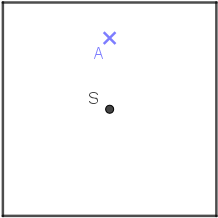
\includegraphics[width=0.3\textwidth]{images/stožnice/folding_kroznica_1.png}
    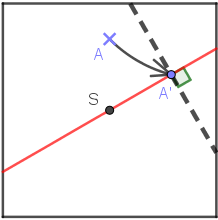
\includegraphics[width=0.3\textwidth]{images/stožnice/folding_kroznica_2.png}
    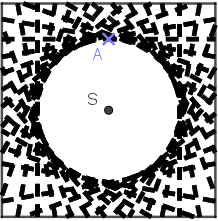
\includegraphics[width=0.3\textwidth]{images/stožnice/folding_kroznica_3.png}
    \caption[Prepogibanje krožnice]{Sukanje izbrane točke okoli središča.}
    \label{fig:koraki_kroznica}
\end{figure}

\opomba{V podpoglavju~\ref{zrcaljenje_origami} smo se naučili prenašati razdalje, zato je zgornja konstrukcija mogoča, zahteva pa še nekaj dodatnih vmesnih pregibov (gl.\ dokaz trditve~\ref{trd:prenasanje_razdalj}).}

Iz konstrukcije pregiba kot pravokotnice na premico $SA'$ skozi točko $A'$ je naslednja trditev očitna in ne potrebuje zapisanega dokaza.

\begin{trditev}
    Konstrukcija iz zgornje aktivnosti nam poda pregib, ki je tangenten na krožnico s središčem v točki $S$ in polmerom $SA$.
\end{trditev}

Za različno izbiro premic skozi točko $S$ dobimo različne tangente in s tem lomljeno krivuljo. S ponavljanjem konstrukcije tangente v neskončnost je krivulja vedno bolj gladka in podobna krožnici.

\subsection{Parabola}

\textit{\textbf{Aktivnost:} Vzemi pravokoten list papirja in svinčnik ter nekje sredi spodnje polovice lista s pisalom označi točko. Nato si izberi točko še na spodnji stranici lista in ga prepogni tako, da se obe izbrani točki prekrijeta. To ponovi čimvečkrat za različno izbiro točke na spodnji stranici papirja (gl.\ sliko~\ref{fig:koraki_parabola}). Kaj opaziš?}

\begin{figure}[h]
    \centering
    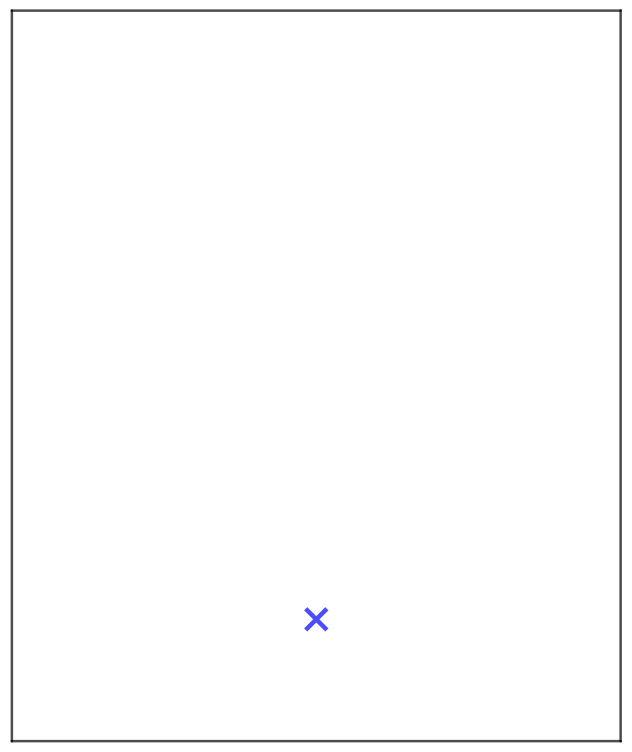
\includegraphics[width=0.3\textwidth]{images/stožnice/folding_parabola_1.png}
    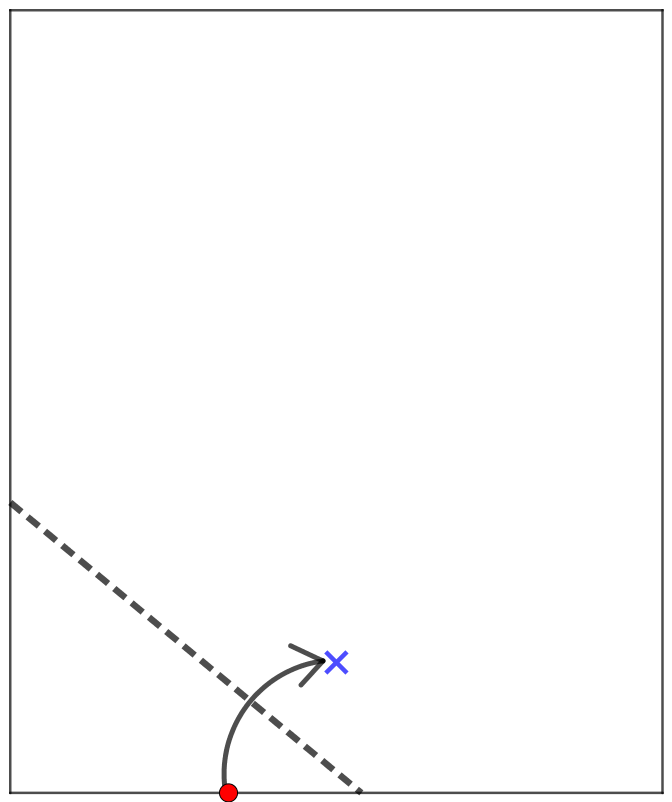
\includegraphics[width=0.3\textwidth]{images/stožnice/folding_parabola_2.png}
    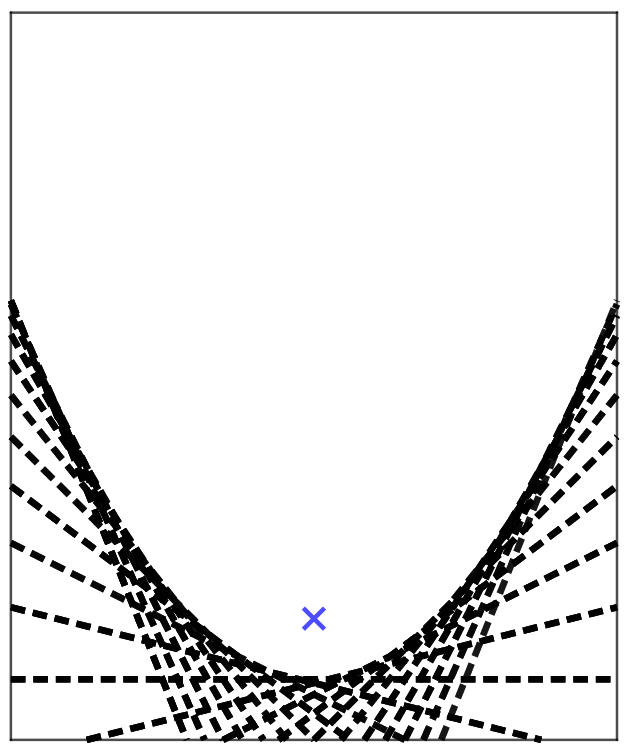
\includegraphics[width=0.3\textwidth]{images/stožnice/folding_parabola_3.png}
    \caption[Prepogibanje parabole]{Prepogibanje spodnje stranice papirja na izbrano točko.}
    \label{fig:koraki_parabola}
\end{figure}

% Najstareši opis zgornje konstrukcije, ker sem jih našla, je v svojo knjigo \emph{Geometric Exercises in Paper Folding} vključil indijski matematik T.\ Sundara Row~\cite{row1917}.
% Hull je našel Row-a (prvič izdana 1893) kot najstarejši zapis te konstrukcije

Omenjen pregib je origami operacija~\ref{op:O3}, lahko pa nanjo gledamo tudi kot na operacijo~\ref{op:O6}. Za le-to smo v poglavju~\ref{pogl:aksiomi} že premislili, da nam pregib, ki poteka skozi dano točko $B$ in točko $A$ položi na premica $a$, poda tangento na parabolo z goriščem $A$ in premico vodnico $a$ (gl.\ sliko~\ref{fig:O6_parabola} in premislek nad njo). Tukaj pa take točke $B$ ni, kar pomeni le to, da smo s pregibom konstruirali neko tangento -- pregib je namreč simetrala daljice, ki ima za krajišči obe izbrani točki iz navodila aktivnosti, torej obstaja točka (točka $P$ na sliki~\ref{fig:O6_parabola}), ki je enako oddaljena od spodnje stranice lista in prve izbrane točke. Nadaljni premislek, da je to edino presečišče pregiba in parabole, je enak kot prej. Spodnja trditev je tako že dokazana.

\begin{trditev}
    Konstrukcija iz zgornje aktivnosti nam poda pregib, ki je tangenten na parabolo z goriščem v izbrani točk in premico vodnico, ki jo predstavlja spodnja stranica lista.
\end{trditev}

Kaj se po večkrat izvedenih pregibih spodnje stranice lista na začetno izbrano točko na papirju izriše? Ker so pregibi tangente na parabolo, predvidevamo, da je izrisana krivulja ravno to. Preden pa to dokažemo, pa poiščimo enačbo teh tangent.

V ta namen si -- brez škode za splošnost, saj lahko z origamijem zrcalimo in rotiramo točke ter premice -- model poljubne točke in  spodnje stranice lista natančno določimo. Uporabimo že znan model iz dokaza izreka~\ref{izr:origami_konstruktibilnost} (pri konstrukciji $\sqrt{r}$): vzemimo točko $A(0, 1)$ in premico $a: y = -1$, ki sta origami-konstruktibilni, in naredimo pregib, ki točko $A$ preslika na premico $a$ v točko $A'(t, -1)$ za nek $t \in \R$ (slika~\ref{fig:enacba_tangente_par1}).

\begin{figure}[h]
    \centering
    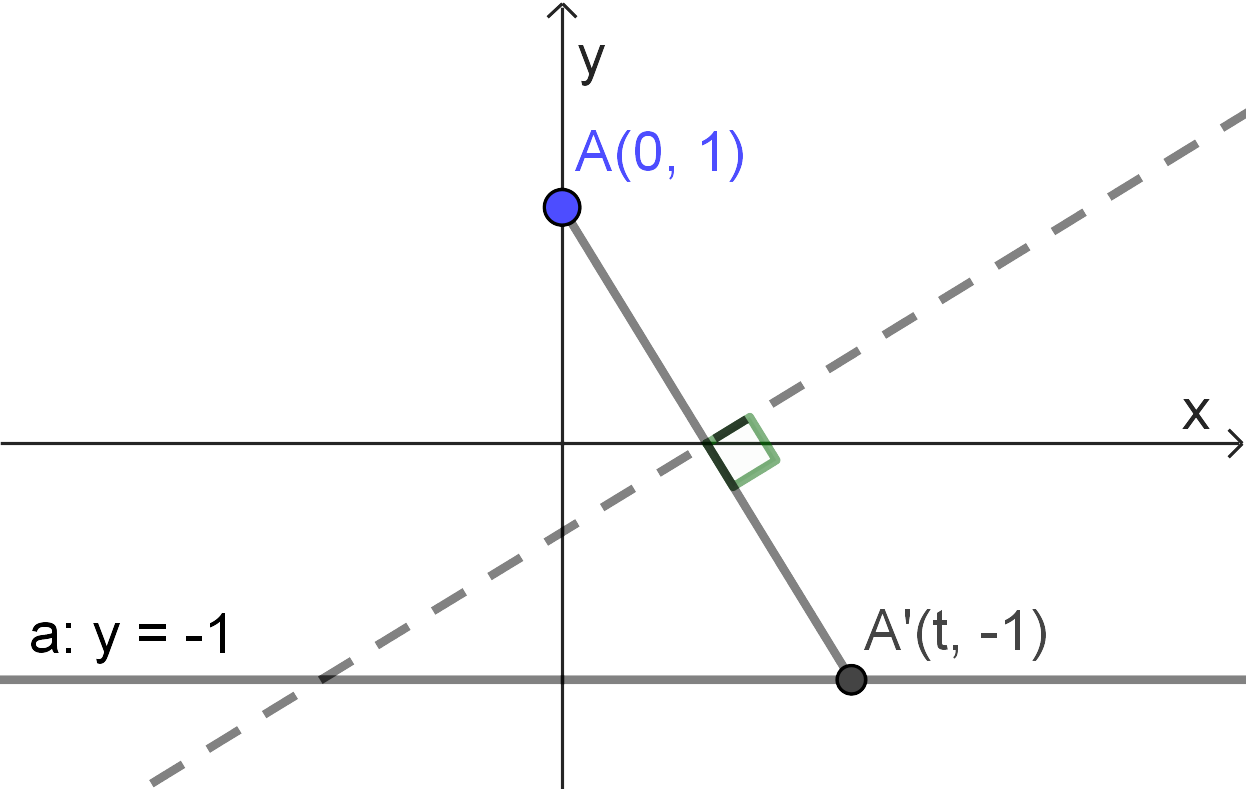
\includegraphics[width=0.5\textwidth]{images/enacba_parabole1.png}
    \caption[Enačba tangente na parabolo]{Pregib točke $A(0, 1)$ na premico $a: y = -1$.}
    \label{fig:enacba_tangente_par1}
\end{figure}

\textcolor{red}{Opcija je tudi, da vseeno malo bolj posplošimo in namesto 1 damo $c$, iz česar se pol lahko tut opazuje, kaj se dogaja, če gorišče bolj odmaknemo od premice vodnice ali pa ji ga približujemo.}

Ker je pregib oz.\ konstruirana premica simetrala daljice $AA'$, lahko hitro določimo njeno enačbo. Koeficient nosilke daljice $AA'$ je $k_A = -\frac{2}{t}$, središče pa $(\frac{t}{2}, 0)$. Tako hitro določimo enačbo pregiba:
\begin{equation}
    y = \frac{t}{2} x - \frac{t^2}{4}.
    \label{eq:tang_par}
\end{equation}
Dobili smo parametrizacijo neke družine premic. Za vsak $t \in \R$ torej dobimo drugo tangento na parabolo z goriščem v točki $A$ in premico vodnico $a$, ki ima zgornjo enačbo.

Za vse točke na pregibu velja, da so enako oddaljene od točk $A$ in $A'$. Vemo že, da obstaja le ena točka $T \in a$, za katero velja $d(T, A) = d(T, a)$. Njena abscisa je $x = t$ (točka $T$ leži na pregibu točno nad točko $A'$) in iz enačbe~\ref{eq:tang_par}, dobimo še ordinato $y = t^2 / 4$. Ker točka $T$ za vsak $t \in \R$ leži na paraboli, pri menjavi $x = t$ dobimo njeno enačbo: $y = x^2 / 4$.

Vendar to ni dokaz, da je obris pregibov iz naloge res parabola. Zgornji premislek temelji na že znanem dejstvu, da so pregibi tangentni na parabole, vendar nam nič ne zagotavlja, da take točke $T$ ležijo točno na obrisu. \textcolor{red}{(A mogoče je tam na strani 56 (Hull2013) spodej, ENVELOPE WAY, kakšen izrek, da ti tangente na ktrivuljo izrišejo prou to krivuljo?)}

Hull v~\cite[str.\ 55--56]{hull2013} poda prefinjen dokaz preko kvadratne formule. Vemo, da pregib~\ref{op:O6} ne obstaja vedno (slika~\ref{fig:O6} desno). Poglejmo, ali obstajajo v ravnini našega modela kakšne točke, skozi katere ne moremo konstruirati pregiba oz.\ tangente. Vzemimo našo parametrizacijo družine tangent (enačba~\ref{eq:tang_par}). Če jo rešimo za $t$, nam dobljena formula pove, za katere vrednosti $t$ pregib poteka skozi točko $(x, y)$:
$$ \frac{1}{4}t^2 - \frac{x}{2}t + y = 0 \Rightarrow t_{1,2} = \frac{\frac{x}{2} \pm \sqrt{\frac{x^2}{4} - y}}{\frac{1}{2}}.$$
Enačba ima dve realni rešitvi pri pogoju $x^2 / 4 - y > 0$, kar pomeni, da vsako točko $(x, y)$, za katero ta pogoj velja, sekata dva pregiba. To so ravno točke pod parabolo $y = x^2 / 4$. Za točke \emph{na} paraboli velja $y = x^2 / 4$, iz česar dobimo eno rešitev $t = x$, torej to točko seka natanko en pregib. Nazadnje nam ostane še območje, za katerega velja $y > x^2 / 4$, t.\ j.\ območje nad parabolo $y = x^2 / 4$, kar nam ne poda realnih rešitev za $t$, torej ga ne seka noben izmed konstruiranih pregibov. Tako je obris, ki ga dobimo v nalogi, res parabola $y = x^2 / 4$.

Torej je naš razmislek dva odstavka višje utemeljen. Sedaj, ko vemo, da je obris, ki nastane po večkratnem prepogibu spodnje stranice lista papirja na izbrano točko, res parabola, lahko pogledamo še več načinov za določitev enačbe parabole~\cite[str.\ 55--56]{hull2013}:
\begin{itemize}
    \item Naj bo $y(x)$ naša parabola, katere enačbo iščemo. Vemo, da je v našem modelu za poljuben $t \in \R$ pregib v neki točki $(x, y(x))$ tangenten na parabolo, koeficient tangente pa je $t / 2$. Očitno velja $x = t$, torej je koeficient kar $x / 2$. Zato dobimo
    $$ \frac{dy}{dx} = \frac{x}{2} \Rightarrow y = \frac{x^2}{4} + C. $$
    Ker parabola očitno poteka skozi točko $(0, 0)$, je $C = 0$ in dobimo želeno enačbo $y = x^2 / 4$.
    \item \textcolor{red}{Envelope way -- gl.\ ~\cite[str.\ 56 spodaj]{hull2013} (tema iz diferencialne ali algebraične geometrije). Gl.\ tudi sliko~\ref{fig:envelope}}
\end{itemize}

\begin{figure}[h]
    \centering
    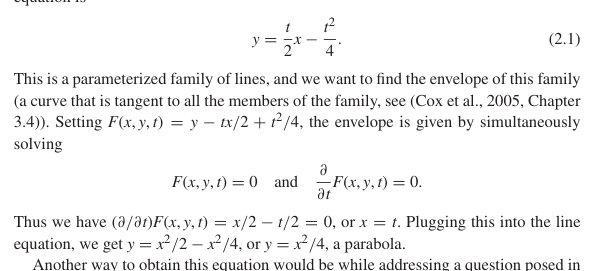
\includegraphics[width=0.5\textwidth]{images/hull2020_envelope_way.png}
    \caption[Envelope]{Izsek iz~\cite[str.\ 32]{hull2020}.}
    \label{fig:envelope}
\end{figure}

\textcolor{red}{na koncu še O7 -- konstrukcija skupne parabole na dve paraboli -- a se da iz tega še kaj pametnega izcimit?}

Aktivnosti za naslednji dve podpoglavji sta enaki kot v tem, le da namesto spodnje tranice lista v izbrano točko prepogibamo krožnico.

\subsection{Elipsa}

\textit{\textbf{Aktivnost:} Vzemi list papirja in svinčnik ter na sredini nariši poljubno krožnico. Označi njeno središče. Na notranji strani krožnice si izberi poljubno točko. Izberi si točko na krožnici in list prepogni tako, da se obe izbrani točki prekrijeta. To ponovi čimvečkrat za različno izbiro točke na krožnici (gl.\ sliko~\ref{fig:koraki_elipsa}). Kaj opaziš?}

\begin{figure}[h]
    \centering
    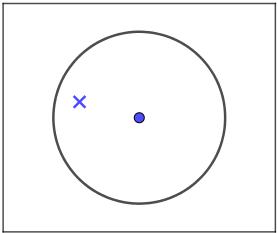
\includegraphics[width=0.3\textwidth]{images/stožnice/folding_elipsa_1.png}
    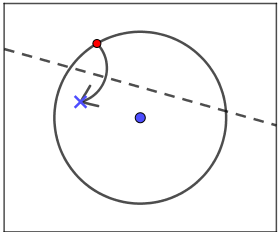
\includegraphics[width=0.3\textwidth]{images/stožnice/folding_elipsa_2.png}
    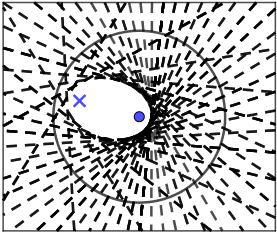
\includegraphics[width=0.3\textwidth]{images/stožnice/folding_elipsa_3.png}
    \caption[Prepogibanje elipse]{Prepogibanje krožnice na izbrano točko znotraj nje.}
    \label{fig:koraki_elipsa}
\end{figure}

\opomba{Za izris poljubne krožnice tu lahko uporabimo šestilo. Prej smo videli, da znamo lomljeno krožnico prepogniti tudi z origamijem, vendar imamo potem na listu papirja veliko pregibov, ki nam ovirajo pogled na ciljno sliko. Zato je uporaba šestila v ta namen dovoljena predvsem iz praktičnega vidika.}

Izgleda, kot da se nam izriše elipsa, ki ima za gorišči središče krožnice in izbrano točko znotraj nje. Spomnimo se, da na elipsi ležijo vse točke, katerih vsota razdalj do obeh gorišč je konstantna in enaka dolžini velike osi (t.\ j.\ dvakratnik velike polosi). V našem primeru je elipsa natančno določena, kar nam pove naslednja trditev~\cite[str.\ 60--61]{hull2013}.

\begin{trditev}
    Konstrukcija iz zgornje aktivnosti nam poda pregib, ki je tangenten na elipso z goriščema v obeh izbranih točkah in veliko osjo, enako polmeru izbrane krožnice.
\end{trditev}

\begin{dokaz}
    Naj bo točka $F_1$ središče krožnice s polmerom $r$ in točka $F_2$ poljubna točka znotraj krožnice. Potem je elipsa, ki ima ti dve točki za svoji gorišči in veliko os enako $r$, natančno določena. Po navodilih iz aktivnosti konstruiramo en pregib, pri čemer na krožnici izberemo poljubno točko $A$ (slika~\ref{fig:dokaz_elipsa} levo). Dokazujemo, da je tangenten na to elipso.

    Označimo s $T$ presečišče pregiba in daljice $AF_1$ (slika~\ref{fig:dokaz_elipsa} na sredi). \textcolor{red}{(Ali presečišče vedno obstaja? Ja, samo še dokaži to)} Ker je pregib simetrala daljice $AF_2$, velja $|TA| = |TF_2|$, torej je
    $$|TF_1| + |TF_2| = |TF_1| + |TA| = |F_1A| = r$$
    za vsako izbiro točke $A$. Ker je $r$ velika os elipse, točka $T$ leži na njej.

    Pokažimo, da je to edino presečišče pregiba z elipso. Naj bo $P$ poljubna točka na pregibu, različna od $T$ (slika~\ref{fig:dokaz_elipsa} desno). Ker leži na pregibu, velja $|PF_2| = |PA|$ in iz trikotniške neenakosti sledi $|PF_1| + |PF_2| = |PF_1| + |PA| > |F_1A| = r$, torej točka $P$ ne leži na elipsi. Pregib v točki $T$ je res tangenta na elipso.

    \begin{figure}[h]
        \centering
        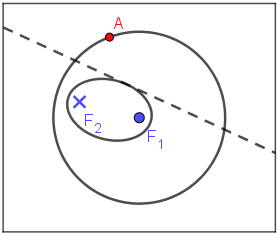
\includegraphics[width=0.3\textwidth]{images/stožnice/elipsa_dokaz1.png}
        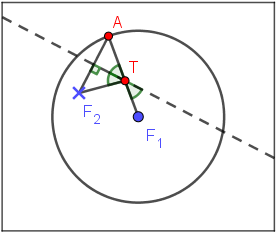
\includegraphics[width=0.3\textwidth]{images/stožnice/elipsa_dokaz2.png}
        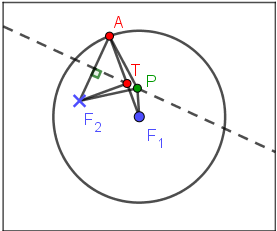
\includegraphics[width=0.3\textwidth]{images/stožnice/elipsa_dokaz3.png}
        \caption[Tangentnost na elipso]{Dokaz tangentnosti pregibov na elipso.}
        \label{fig:dokaz_elipsa}
    \end{figure}  
\end{dokaz}

Bolj analitičen dokaz, kjer se izračuna splošno enačbo te elipse glede na izbrano krožnico in točko znotraj nje, najdemo v~\cite[str.\ 204--205]{smith2003}.

\textcolor{red}{še dokaz, da je OBRIS elipsa, kot prej s parabolo npr.\ iz kvadratne enačbe? Referenca na dokaz je v~\cite[str.\ 60]{hull2013}. Pa mogoče ista fora z ogrinjačami kot pri paraboli?}

Kaj pa, če pri konstrukciji izberemo točko izven krožnice?

\subsection{Hiperbola}

\textit{\textbf{Aktivnost:} Vzemi list papirja in svinčnik ter na sredini nariši poljubno krožnico. Označi njeno središče. Na zunanji strani krožnice si izberi poljubno točko. Izberi si točko na krožnici in list prepogni tako, da se obe izbrani točki prekrijeta. To ponovi čimvečkrat za različno izbiro točke na krožnici (gl.\ sliko~\ref{fig:koraki_hiperbola}). Kaj opaziš?}

\begin{figure}[h]
    \centering
    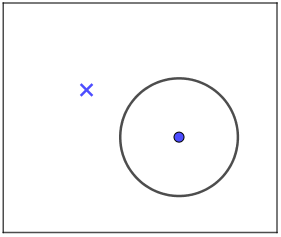
\includegraphics[width=0.3\textwidth]{images/stožnice/folding_hiperbola_1.png}
    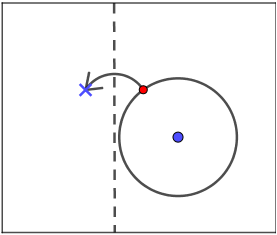
\includegraphics[width=0.3\textwidth]{images/stožnice/folding_hiperbola_2.png}
    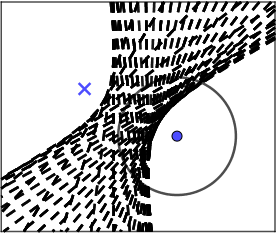
\includegraphics[width=0.3\textwidth]{images/stožnice/folding_hiperbola_3.png}
    \caption[Prepogibanje hiperbole]{Prepogibanje krožnice na izbrano točko zunaj nje.}
    \label{fig:koraki_hiperbola}
\end{figure}

Podobno kot prej lahko sklepamo, da se nam izriše obris hiperbole. Spomnimo se, da na hiperboli ležijo vse točke, katerih absolutna vrednost razlike razdalj do obeh gorišč je konstantna in enaka dolžini velike osi. Tako kot pri elipski je tudi tu hiperbola natančno določena. Naslednja trditev in dokaz sta zato zelo podobna kot za elipso.

\begin{trditev}
    Konstrukcija iz zgornje aktivnosti nam poda pregib, ki je tangenten na hiperbolo z goriščema v obeh izbranih točkah in veliko osjo (t.\ j.\ dvakratnik velike polosi), enako polmeru izbrane krožnice.
\end{trditev}

\begin{dokaz}
    Naj bo točka $F_1$ središče krožnice s polmerom $r$ in točka $F_2$ poljubna točka zunaj krožnice. Potem je hiperbola, ki ima ti dve točki za svoji gorišči in veliko os enako $r$, natančno določena. Po navodilih iz aktivnosti konstruiramo en pregib, pri čemer na krožnici izberemo poljubno točko $A$ (slika~\ref{fig:dokaz_hiperbola} levo). Dokazujemo, da je tangenten na to hiperbolo.

    Označimo s $T$ presečišče pregiba in nosilke daljice $AF_1$ (slika~\ref{fig:dokaz_hiperbola} na sredi). \textcolor{red}{(Ali presečišče vedno obstaja? NE, V 2 PRIMERIH DOBIMO ASIMPTOTO - ko je premica vzporedna k pregibu)} Ker je pregib simetrala daljice $AF_2$, velja $|TA| = |TF_2|$, torej je 
    $$\left||TF_1| - |TF_2|\right| = \left||TF_1| - |TA|\right| = |F_1A| = r$$
    za vsako izbiro točke $A$. Ker je $r$ velika os hiperbole, točka $T$ leži na njej.

    Pokažimo, da je to edino presečišče pregiba s hiperbolo. Naj bo $P$ poljubna točka na pregibu, različna od $T$ (slika~\ref{fig:dokaz_hiperbola} desno). Ker leži na pregibu, velja $|PF_2| = |PA|$ in sledi $\left||PF_1| - |PF_2|\right| = \left||PF_1| - |PA|\right|$. Predpostavimo, da je to enako $r$ in poglejmo, za katere možne položaje točke $P$ je to mogoče:

    \textcolor{red}{Spodnja slikca je ideja, dodelaj da bo natančno. Fora je spet trikotniška neenakost. In da mora P ležat na nosilki $AF_1$ IN pregibu, kar je točno točka T, ki je različna od nje, kar je pač protislovje.}

    \begin{figure}[h]
        \centering
        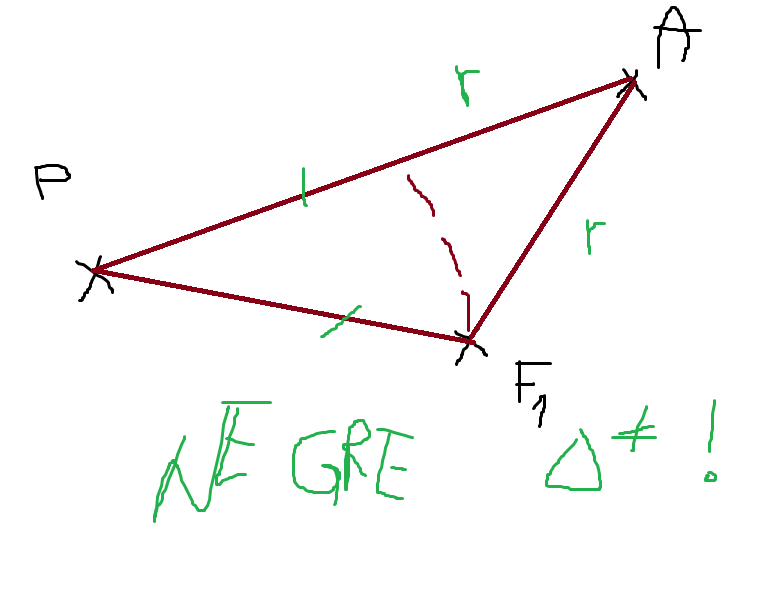
\includegraphics[width=0.5\textwidth]{images/stožnice/hiperbola_dokaz_ideja.png}
    \end{figure}

    \begin{itemize}
        \item Točka $P$ leži na krožnici: Potem je $|PF_1| = r$, iz česar sledita dve možnosti:
            \subitem $|PA| = 0$ oz.\ $P = A$. To pomeni, da pregib poteka skozi točko $A$, kar pa ni mogoče.
            \subitem $|PA| = 2r$ oz. 
        \item Točka $P$ leži znotraj krožnice: 
        \item Točka $P$ leži zunaj krožnice: Potem je $|PF_1| > r$. Če je $|PA| = |PB|$ (kjer je točka $B$ presečišče daljice $PF_1$ s krožnico), pridemo v protislovje s trikotniško neenakostjo, saj dobimo $|PA| + |AF_1| = |PB| + |BF_1| = |PF_1| < |PA| + |AF_1|$. \textcolor{red}{(Naredi slikco kot je na 18ki desno, pa dodaj še točko B)}. Potem lahko velja samo še $|PA| > 2r$. \textcolor{red}{dodelaj}
    \end{itemize}
    
    \textcolor{red}{DOKAŽI, DA NIČ OD TEGA TROJEGA NE GRE!!}
    Ker ne velja nič od tega trojega, točka $P$ ne leži na hiperboli. Pregib v točki $T$ je res tangenta nanjo.

    \begin{figure}[h]
        \centering
        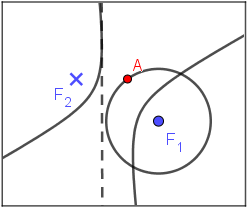
\includegraphics[width=0.3\textwidth]{images/stožnice/hiperbola_dokaz1.png}
        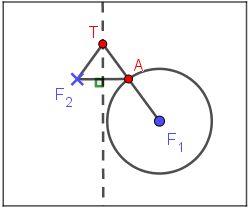
\includegraphics[width=0.3\textwidth]{images/stožnice/hiperbola_dokaz2.png}
        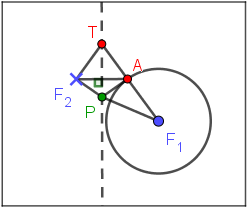
\includegraphics[width=0.3\textwidth]{images/stožnice/hiperbola_dokaz3.png}
        \caption[Tangentnost na hiperbolo]{Dokaz tangentnosti pregibov na hiperbolo.}
        \label{fig:dokaz_hiperbola}
    \end{figure}  
\end{dokaz}

\textcolor{red}{Bolj analitičen dokaz, kjer se izračuna splošno enačbo te hiperbole glede na izbrano krožnico in točko zunaj nje, najdemo v~\cite[str.\ 205--206]{smith2003}. Nekaj je tudi v~\cite[str.\ 34 spodaj]{hull2020}. Lep dokaz za elipso in hiperbolo (oboje skupej) je tudi v~\cite{lotka1907} --`` a very nice analytical method that simultaneously proves that the resulting envelopes are ellipses and hyperbolas''. Pa tudi v~\cite{yates1943} so dokazi ``for the parabola, ellipse, and hyperbola that are the most concise and elegant that the
author has seen''}